 \documentclass[a4paper, twocolumn]{article}
%\documentclass[a4paper]{article}
\makeatletter
\def\@seccntformat#1{%
  \expandafter\ifx\csname c@#1\endcsname\c@section
  \thesection $\mid$
  \else
  \csname the#1\endcsname\quad
  \fi}
\makeatother
\usepackage{tikz}
\usetikzlibrary{positioning,arrows,automata}
\usepackage{abstract}
\usepackage{fullpage}
\usepackage[utf8]{inputenc}
\usepackage[english]{babel}
\usepackage{lipsum}
\usepackage{amsmath}
\usepackage{amsfonts}
\usepackage{pgf, tikz}
\usepackage{pgfplots}
\usepackage{float}
\usepackage{listings}
\usepackage{xcolor}
\usepackage{tabularx}
\usepackage{hyperref}
\usepackage[all]{xy}
\usetikzlibrary{fit,arrows.meta}
\usetikzlibrary{automata, positioning}


% FOR THE CODE IN SECTION 5 
\definecolor{codegreen}{rgb}{0,0.6,0}
\definecolor{codegray}{rgb}{0.5,0.5,0.5}
\definecolor{codepurple}{rgb}{0.58,0,0.82}
\definecolor{backcolour}{rgb}{0.95,0.95,0.92}

\lstdefinestyle{mystyle}{
    backgroundcolor=\color{backcolour},
    commentstyle=\color{codegreen},
    keywordstyle=\color{magenta},
    numberstyle=\tiny\color{codegray},
    stringstyle=\color{codepurple},
    basicstyle=\ttfamily\scriptsize,
    breakatwhitespace=false,
    breaklines=true,
    captionpos=b,
    keepspaces=true,
    numbers=left,
    numbersep=5pt,
    showspaces=false,
    showstringspaces=false,
    showtabs=false,
    tabsize=2
}

\usepackage{titlesec}

\setcounter{secnumdepth}{4}
\titleformat{\paragraph}
{\normalfont\normalsize\bfseries}{\theparagraph}{1em}{}
\titlespacing*{\paragraph}
{0pt}{3.25ex plus 1ex minus .2ex}{1.5ex plus .2ex}

\lstset{style=mystyle}

\title{\textbf{Security analysis of Corona Tracing Applications}}
\date{\textbf{-- BSP6 --}\\ \today}
\author{
    Maria ZHEKOVA\\
    \small University of Luxembourg\\
    \small\texttt{maria.zhekova.001@student.uni.lu}
	\and
    Marjan SKROBOT\\
    \small University of Luxembourg\\
	\small\texttt{marjan.skrobot@uni.lu}
	\and
	Yan KIM\\
	\small University of Luxembourg\\
	\small\texttt{yan.kim@uni.lu}
}

\begin{document}
\maketitle

% ---------- ABSTRACT ---------- 
\begin{abstract}
    \noindent The COVID-19 pandemic has seen governments across the world restricting civil liberties and movement to new levels. To aid the safe lifting of current public health restrictions, new technologies called \textbf{contact tracing apps} are being developed. These apps are rolled out to automate labour intensive tasks, critical to containing the spread of the virus. \\
    In this paper we present the architecture of Corona Tracing Applications with a following analysis and verification of the security goals in such systems. We use model checking to determine whether the security goals hold in a given policy are satisfied. This report uses parts of a given template that can be found in \cite{template}.
\end{abstract}

% ---------- 1| INTRODUCTION ---------- 
\section{Introduction}
The pandemic has set new measures, forcing lockdowns and straining public health care systems. The virus has forced people to instigate strict social distancing criteria in order to decrease the spread of the COVID-19 virus. A COVID-19 positive person may be contagious even without experiencing symptoms. Thus by the time the person tests positive the virus could have been already spread to many others with whom he/she came to contact. In this context, researchers from all over the world have been focusing on Contact Tracing Applications with the aim to quickly and reliably identify contacts that might be at infection risk.\\
There were various propositions on such applications, not only depending on different security and privacy aspects but also on the computing power of such systems. Countries differ in their social norms and values, thus they may embrace different types of Contacts Tracing Systems.\\
Nevertheless, most of them aim to deliver to the population a functional Contact Tracing Application, capable to detect possible people at risk and keep the personal data entered by the user private. However, even in the best Contact Tracing Systems, there are limitations of how private systems can be made, because identifying COVID-19 users is the whole point of these applications.

% ---------- 2| PROJECT DESCRIPTION ---------- 
\section{Project description}
In this paper we introduce the architecture of Corona Tracing Applications and the necessary protocols. We will be using a model checker called Uppaal \cite{uppaal} for the analysis and verification of the application. Uppaal is used for modelling, validation and verification of real-time systems modeled as networks of timed automata. The description of a model in Uppaal consist of three parts: global and local declarations, automata templates and a system definition.


% --------------------  2.1 DOMAINS ---------- 
\subsection{Domains}
In this section we will present the scientific and technical domain of the project.
\subsubsection{Scientific }
The scientific aspect of the bachelor semester project is the research and study of Corona Tracing Applications and their protocols.
In addition, the knowledge of the syntax and semantics of Linear Temporal Logic (LTL) is of great importance.
\subsubsection{Technical}
The technical aspect of this project is the design and implementation of a model in order to provide analysis and verification of Corona Tracing Applications. To do so, the student must learn how to use Uppaal and its specific language.

% --------------------  2.2 TARGET DELIVERABLES ---------- 
\subsection{Targeted Deliverables}
\label{sec-deliverables}
\subsubsection{Scientific deliverables}
The scientific deliverables of the project are several reports and videos containing the study analysis and explanation of the architecture of various Corona tracing applications and protocols, such as DP-3T. In addition they include security properties and important knowledge gathered in order to produce the technical deliverable.
\subsubsection{Technical deliverables}
The technical deliverable is a modelling and verification of security properties of the corona tracing protocol using the model checker Uppaal and following its specification language.


% ---------- 3| PRE-REQUISITES---------- 
\section{Pre-requisites} 
In this section, it will be described the main scientific and technical knowledge that is required to be known before starting the project.

\subsection{Scientific pre-requisites}
As a main scientific knowledge, it is important to have a basic knowledge of common security issues and vulnerabilities. The student needs to know beforehand crucial security aspects such as authentication, authorization and validation.\\
In order to present a sophisticated security analysis, the student must be familiar to oversee systems to stave off potential security breaches. 

\subsection{Technical pre-requisites}
The student must be familiar with automata theory and be able to create and analyse state diagrams of transition systems from where the potential behaviour of tracing apps will be described. These diagrams will help in the modelling of the system in Uppaal.

% ---------- 4| SCIENTIFIC DELIVERABLE ---------- 
\section{Defining a strategy}%(A Scientific Deliverable 1)}
Here it will be explained in details all the important aspects needed in order to come up with the design of the system model before starting to work with Uppaal.
\label{sec-production}

% --------------------  4.1 REQUIREMENTS ---------- 
\subsection{Requirements}
As mentioned before, it is of a crucial importance to have deeper knowledge of the architecture of Corona Tracing Apps, protocols and to understand how they work in order to make analysis and verification of models.\\
Another important requirement is to understand how a system verification can be made and represent the system in a formal language.
% --------------------  4.2 DESIGN ---------- 
\subsection{Background}
In this section will be explained the knowledge gathered during the semester about different types of tracing app architectures, protocols and their security aspects.
\subsubsection{Architectures and Protocols}
The architectures differentiate themselves by having different key attributes, data management, privacy and security management and attack vulnerabilities. The three distinct system architectures which are commonly used or proposed for the development of COVID-19 tracing applications are the  \textbf{centralised}, the \textbf{decentralised} and the \textbf{hybrid} architectures. Each of these architectures has pros and cons, different attack models and protections \cite{survey}.\\
The main actors for each architecture are: users, server, authority/diagnosis facility. An abstract representation of any sort of a corona tracing app may be explained as the following:\\
\textit{Each user has a set of specific ID's or only one ID, used to send to the close-by users as an encounter message. When an user \texttt{A} is labeled as COVID-19-positive from the diagnosis facility, the server may receive all the encounters of \texttt{A} from the last few days, keeping in mind that \texttt{A} should be verified of being COVID-19-positive via the authority.}\\

\noindent There are additional specifications to this explanation which defer, depending on the architecture.\\
We focused our research on the decentralised architecture and the functionalities of the Decentralized Privacy-Preserving Proximity Tracing \texttt{DP-3T} protocol. However it is important to understand the difference between the different architectures before continuing further.\\

% --------- CENTRALIZED --------- 
\noindent \textbf{Centralized with BlueTrace protocol}\\
In the centralized architecture, the server is involved in most of the tasks.\\
Upon registration of a new user, the server receives information such as telephone number, name, postcode, etc. After confirmation with One-Time-Password (OTP) the user receives a \texttt{TempID}, encrypted with an individual secret key only known to the server. This \texttt{TempID} is then used in the encounter message altogether with the model of the phone and Transmit Power (TxPower) kept in the beacon of the Bluetrace protocol. A new \texttt{TempID} is generated by the server around every 15 minutes.\\
The encountered messages are stored in each device with the time received and the Received Signal Strength Indicator (RSSI) used for determining the distance between two users.\\
When an user tests positive for COVID-19, the authority verifies if there is a registration made in the application and if there is a match, the user is flagged as infected. The user chooses to either upload its encounter data, called \texttt{seeds} or not to the server. If the user chooses to upload the encountered messages, there is a verification process and upon success. The server decrypts the encountered \texttt{TempIDs} with their Individual secret key and prepares a list depending on the distance of proximity which is calculated with the information from TxPower and RSSI. Then, when an user chooses to download the seeds from the server. All of the COVID-19 positive seeds are downloaded and the user is notified if there has been a contact with COVID-19 positive tested user.\\

\noindent In theory, a personal information is not transmitted in this encounter message, but the message still can be exploited by a skilled attacker. For instance, an attacker could exploit weaknesses based on the model of the smartphone and launch an attack.\\
The survey, from which we are gathering our information does not mention if this secret key is to be regenerated every now and then but we assume it is, because if the individual secret key is not regenerated this could be very dangerous. If an attacker finds a way to extract the keys from the server, there will be leak of information such as name, phone number, ZIP code and age range. There would be a risk of a possible false data injection if the attacker proceeds further. Hence, the attacker could flag someone to be of a proximity with a COVID-19 positive user or even to be COVID-19 positive, if the server gets further compromised.\\

% --------- DECENTRALIZED --------- 
\noindent \textbf{Decentralized with Private Automated Contact Tracing (PACT) protocol}\\
In the decentralised architecture, most of the tasks are done by the user's device and the server is little involved.\\
For instance, users are not required to register and thus there is not storage of name, nor phone number, etc. Devices generate randomly seeds every hour with a pseudo-random function, and with them, the so called \texttt{chirps} are generated. These chirps are broadcasted via Buetooth every few seconds anonymously. New chirps are generated every 1 min allowing to decrease the possibility of tracking. When user receives chirps, they are stored with a timestamp and the maximum RSSI value.\\
If an user is diagnosed as COVID-19 positive, the authority gives unique permission number which allows the user to upload all of the stored seeds altogether with the validity period (expiry times of seeds and creation time of seeds). The server gets all the seeds associated with the user.\\
When user wants to download any seeds, uploaded by infected user, they are reconstructed with the pseudo-random function to produce a risk analysis.\\

\noindent There are no obvious privacy risks as in the centralized architecture since there is no personal data given to the server.\\
It is important to note that one of the main differences between the two architectures is that in the decentralized, the server receives the seeds associated with a single identified user and in the centralized, the server receives the complete contact list of all users in a proximity.\\
The decentralized architecture is less vulnerable to tracking attacks since new chirps are generated every 1 minute. But it is however not completely secure as nothing is completely secure and a skilled adversary could find a back door and exploit weaknesses.\\

% --------- HYBRID --------- 
\noindent \textbf{Hybrid}\\
The hybrid architecture is as the name suggests a mix between centralized architecture and decentralized architecture. Here the tasks are split up between the device and the server. The \texttt{TempID} generation is done by the device. The server has no statistical information that later on could be exploited by a malicious attacker.\\
In this architecture, the user needs to register, but the server does not store the phone number, nor model. Upon validation with OTP, the phone number is permanently deleted. The server then, generates an unique ID and generates an encryption key and sends both to the app of the user. The encryption key is permanently deleted from the server but the ID is kept, since the user will be identified with it.\\
The app maintains two tables: \texttt{upload} table and \texttt{query} table. Each 15 minutes an ephermal identifier called \texttt{EphID} is generated with the Diffie Hellman key exchange mechanism \cite{diffie} and broadcasted. When user receives an \texttt{EphID}, two \texttt{PET}s are generated. One of them is stored the query table and the other in the upload table altogether with the timestamp and duration. The \texttt{PET}s are defined as the following: \\
$PET_1 = H('1'|g^{a\cdot b})$ and $PET_2 = H('2'|g^{a\cdot b})$ \\
The information in the tables are stored hash functions which decrease the leak of information if a device is compromised.\\
If an user is tested COVID-19 positive, it sends to the server the \texttt{ID}, the encryption key and the upload table.\\
In this architecture, users do not download information from the server. If an user wants to verify if there was an exposure with an infected person, the user uploads as well its upload table. At this stage, the server produces risk analysis, and informs the user about the result.\\

\noindent For each architecture there is a set of specific protocols which can be found in the map representation on Figure \ref{fig:setProt} of Section \ref{appendix}.\\

\noindent Each country, where a contact tracing app is authorized chooses the type of architecture. Until now the hybrid systems are still not fully verified and validated although they seem to be more secure. Therefore the world is split up in-between the centralized and decentralized choice.\\
Each system has its vulnerabilities. If the encounter messages in the centralized architecture leak, the identity of user and his/hers contacts is reveled but the adversary could be only the server. If the encounter messages in the decentralized system leak, only the identity of the user leaks, but the adversary could be anyone \cite{orOr}.\\

\noindent As stated before, the center of our research is the decentralized architecture with the DP-3T protocol. Here we will introduce briefly the DP-3T protocol and its properties \cite{dp3t-white}\cite{dp3t}. \\

\noindent \textbf{DP-3T protocol}\\
This is an open protocol developed specially in response to the COVID-19 pandemic. It uses Bluetooth Low Energy to track and log encounters. In this protocol the server does not have access to contact logs nor it is responsible for processing and informing clients that they were in contact of a COVID-19 positive user. Hence, the contacts are never transmitted to third parties, which benefits of privacy. However, it requires more computing power on the user's device in order to process infection reports.\\
The participants of the DP-3T system are; users, a back-end server and a health authority. The back-end server keeps the data that needs to be pushed by smartphones when they are authorized by the authority.\\
There are three types of the protocol: low-cost, unlinkable and hybrid. As the name suggest, the low-cost type has very small bandwidth requirements. The unlinkable type, on the other hand offers better privacy properties but increased bandwidth. The hybrid design is the combination of both.\\
\textbf{Low-cost:}\\
The app creates a \texttt{$SK_0$} key with a length suggested to be \texttt{HMAC-SHA256}, which means that the key length cannot be less than 32 bytes. Each day this key is generated by computing \texttt{$SK_t = H(SK_{t-1})$} with $t$ being the current day and $H$ a cryptographic function. The \texttt{EphID} is generated with the help of this \texttt{$SK_t$} key.\\
During encounters, the phone stores the received \texttt{EphID}, exposure measurement and the day on which it was received.\\
When user is diagnosed with COVID-19 and validated by the health authority, the user can upload to the backed of the server the seed \texttt{$SK_t$} and $t$, corresponding to the first day, the user is considered contagious. After sending it, the smartphone deletes it and generates randomly new one. Since the seed (\texttt{$SK_t,t$}) is uploaded, each user downloading the infected (\texttt{$SK_t,t$}) pairs from the server can verify if there was an encounter on the day $t$ with the \texttt{EphID} of each, which is reconstructed with \texttt{$SK_t$}.\\
\textbf{Unlinkable:}\\
The unlinkable design is similar to the preivous one.\\
During encounters, the phone does not store the plain \texttt{EphID}, but a hashed string of it:\\ \texttt{H(EphID || i)}, where \texttt{i} is the epoch in which the beacon is received. This is used to create a so called a \texttt{Cuckoo} filter. In this type of DP-3T, the phone stores also the exposure measurements and the day $t$.\\
\textbf{Hybrid:}\\
Here the devices generate random seeds for each time window and use them similarly to the low-cost design. Depending on the length of the window, this design offers better protection against linking \texttt{EphIds} for all epoch but the protection against tracking is weaker than with the unlinkable design. This design is very similar to the \texttt{Google/Apple} design.\\

\noindent \textbf{Apple/Google Exposure Notification project}\\
The Apple/Google design \cite{appGoog} uses one seed to generate \texttt{EphIDs} of the day and thus corresponds to the time window of 1 day. The \texttt{EphID} change every 10-20 minutes. The procedure is similar to the DP-3T protocol.\\

\noindent The analysis document of DP-3T from Serge Vaudenay \cite{analyDP3t} argues that some privacy protection measurements by the DP-3R protocol may have the opposite effect. Hence, the so called \texttt{private} encounters may be revealed.

\subsubsection{System verification} \label{sysVerif}
The verification of a system is a very important step that needs to be always executed. In this document, we are basing our knowledge on a book for principles of model checking \cite{book}.\\
There could be a hardware and software errors in a system, hence both should be verified. In this book, a very interesting and dramatic example is given for the importance of system verification.\\
In June 1996, there was a fault in the control software of the Ariane-5 missile due to a conversation of a 64-bit floating point into a 16-bit integer value, which caused complete loss of guidance, altitude information and explosion just forty seconds after its lift-off. Similar software was used in systems such as nuclear power plants, traffic control and alert systems. A very small mistake in the configuration could be fatal.\\
It is proven that the verification process takes more time than the actual construction of the software or hardware. Therefore, there exist several techniques to facilitate the process. One of them is the goal the this project: the model checking.\\
Formal methods are used to describe mathematically a possible system behaviour. There exist software for model checking which based on a correct implementation explore all possible system states in a brute-force manner.\\
There is defined a specific process for model checking with three phases:
\begin{itemize}
    \item \textbf{Modeling phase} - modeling the system using the language of the model checker (often similar to \texttt{C}/\texttt{C++}), then performing some simulations to see if it runs smoothly and lastly define a property using the property specification language.
    \item \textbf{Running phase} - here the property defined in the previous phase should be verified.
    \item \textbf{Analysis phase} - if the property is satisfied, the verifier must define and check for another property; if the property was violated, an analysis should be made in order to refine the model and repeat the entire procedure.
\end{itemize}
A graph explaining the path of each technique can be found in Figure \ref{fig:modelCheck} of Section \ref{appendix}.

\subsubsection{Modelling concurrent systems}
Here we will quickly introduce the topic since the principles could cover immense part of the report, more detailed explanation could be found in \cite{book}.
The behaviour of a system is often defined by transition systems (TS). They are very similar to automaton diagrams, where nodes represent states and the edges are model transitions. The state of the system describes the behaviour in a  certain moment.\\
A transition system is a tuple $(S, Act, \rightarrow , I,AP,L)$ where
\begin{itemize}
    \item $S$ is a set of states,
    \item $Act$ is as set of actions
    \item $\longrightarrow \subseteq S \times Act \times S$ is a transition relation,
    \item $I \subseteq S$ is a set of initial states,
    \item $AP$ is a set of atomic propositions,
    \item $L : S \rightarrow 2^{AP}$ is a labeling function
\end{itemize}
If $S, Act$ and $AP$ are finite, the TS is called finite.\\
Depending on the number of variables or components, the size of TS representation grows exponentially.\\

\noindent There are different types of automatons.\\
In a \textbf{Deterministic Finite Automaton (DFA)} there is only one state transition for each symbolic representation of the alphabet.It cannot use empty string transition and a dead state is required. It is also non deterministic and rejects the string in case it terminates in a state different from the accepting state.\\
In a \textbf{Non deterministic Finite Automaton (NFA)} there is no specification of how does the NFA reacts according to a symbol of the alphabet. A dead state is not required, not all NFA are DFA and rejects the string in the event of all branches dying or refusing the string.

\subsubsection{Linear-Time Properties (LTP)}
In this section we will introduce briefly the properties of interest that should be verified.\\
One important property is the \texttt{deadlock}. The deadlock occurs when the system is in a terminal state and one element is in a non terminal state. When this happens, the whole system comes to a halt. Often a deadlock occurs when components mutually wait for each other to finish.\\
There are two types of approaches for analysing a computer system: action-based approach and state-based approach. In the action based approach only action labels of the transition are taken into consideration and it is only necessary for modelling communication. The state-based approach looks only into the labels in the state sequences.\\
The LTP specify the traces that a TS should only exhibit. Therefore it specifies the admissible behaviour of the system.\\
A more formal definition of a LTP is:\\
\colorbox{backcolour}{\texttt{A linear-time property}}\\
\colorbox{backcolour}{\texttt{$P$ over $AP$ is a subset of $(2^{AP})^w$}}\\
LPT is a set of language of infinite words over the alphabet $2^{AP}$, thus $(2^{AP})^w$ stands for the set of words in $2^{AP}$.\\
There exist also the so called \texttt{safety properties}, where for instance a deadlock does occur. This is called an \texttt{invariant} property. This invariant is given by a certain condition for the states and requires that this condition holds for all reachable states.\\
Safety properties are complemented also by \texttt{liveness} properties that require some progress. This is the inverse of the \texttt{invariant}. For instance a good example for a liveness property is that a program should eventually terminate.\\
There are three key words for the liveness properties: \texttt{eventually}, \texttt{repeated eventually} and \texttt{starvation freedom}. In a latest section we will see the specification for these properties in \texttt{Uppaal}. They will help us formulate the query language for the formal verification of the model.

% --------------------  4.3 PRODUCTION ---------- 
\subsection{Formalization and Visualization} \label{formVis}
Our main goal was to be able to verify a COVID-19 tracing app in Uppaal. Therefore we used an already implemented LTL formal representation of a part of such decentralized system for direction orientation \cite{formalization}.\\
In this section we will represent the used components from \cite{formalization} and the designed graph for later use of direction for the automaton in Uppaal. An important remark is that in the document, the authors abstract away from physical locations and model physical contact using non-determinism. They select at each step the set of users that receive the identifier broadcasted by the app. We will have a slightly different approach.\\
If we were to use the setting from the document we would define the following:
\begin{itemize}

    \item \texttt{$t$} for the current time
    \item \texttt{q $\in$ {0,1,2}} for the COVID-19 status, where \texttt{0} is for negative, 1 is for possibly positive and 2 is for positive.
    \item \texttt{$u$} is the user's id
    \item \texttt{$e$} is the current valid ephermal id (\texttt{EphID})
    \item \texttt{$S$} is the set of sent \texttt{$e$} by \texttt{$u$} 
    \item \texttt{$R$} is the set of received \texttt{$e$} by \texttt{$u$} 
    \item \texttt{G} for the server
    \item \text{$\Delta$} for the set of user states
    \item \texttt{$\delta$} is the state of the user
\end{itemize}
The contact tracing system will be defined as the tuple \colorbox{backcolour}{$< G, \Delta, t >$}.\\
The state of an user is represented as the tuple \colorbox{backcolour}{$\delta = < q,u,e,t,S,R >$}. A new state is defined by \texttt{$\delta`$}\\
Therefore, we can design a proposition for automaton representation of only one \texttt{EphID} generation and a second generation when the user is tested COVID-19 positive. This proposition is found below in Figure \ref{fig:usr}.
\begin{figure}[H]
    \centering
    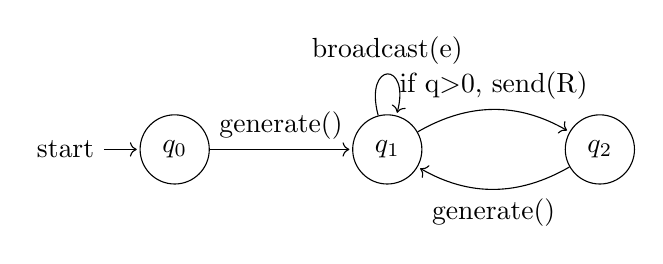
\begin{tikzpicture}[shorten >=1pt,node distance=2.7cm,on grid,auto]
        \node[state,initial] (q0) {$q_0$}; 
        \node[state, right of=q0] (q1) {$q_1$}; 
        \node[state, right of=q1] (q2) {$q_2$};
        \path[->] 
                (q0) edge[above] node{generate()} (q1)
                (q1) edge[loop above] node{broadcast(e)} (q1)
                (q1) edge[bend left, above] node{if q$>$0, send(R)} (q2)
                (q2) edge[bend left, below] node{generate()} (q1);
    \end{tikzpicture}
    \caption{User}
    \label{fig:usr} 
\end{figure}
\noindent This representation is only on the level of the user and not in the application level and there is an assumption that the application is already installed. It is a very simple representation which we are using to build on and design the more broad generation of ephermal ids.
\begin{itemize}
    \item \textbf{q0 - q1}: the ephermal id \texttt{e} is generated
    \item \textbf{q1 - q1}: broadcast (send and receive)
    \item \textbf{q1 - q2}: if the user \texttt{u} is tested COVID-19 positive or possible positive aka \texttt{q>0}, the received ephermal ids \texttt{R(e)} are sent to the Authorities 
    \item \textbf{q2 - q1}: generation of a new ephermal id \texttt{e}
\end{itemize}
The automaton representation of the authority is similar to the following:\\
\begin{figure}[H]
    \centering
    \begin{tikzpicture}[shorten >=1pt,node distance=3cm,on grid,auto]%[node distance=3cm]
    \node[state, initial, left of=q0] (q0) {$q_0$}; 
    \draw   (q0) edge[loop above] node{if valid,send(R)} (q0);
    \end{tikzpicture}
    \caption{Authority}
    \label{fig:authority} 
\end{figure}
\noindent As seen in the last sections, the role of the Authority differs a bit. On Figure \ref{fig:authority} we represent the authority as having the role to verify if the user's ID is COVID-19 positive and add it to the list of infected users on the Server. Where the number of the user is verified and if it is valid, the set of received ephermal IDs is added to the data.\\
\begin{figure}[H]
    \centering
    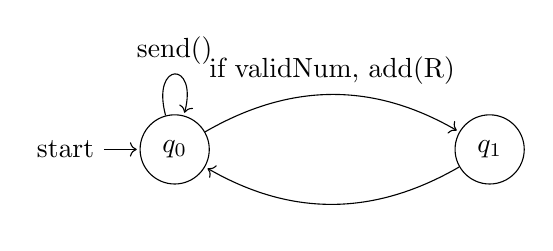
\begin{tikzpicture}[shorten >=1pt,node distance=4cm,on grid,auto]%[node distance=3cm]
    \node[state,initial] (q0) {$q_0$}; 
    \node[state, right of=q0] (q1) {$q_1$}; 
    \path[->] 
            (q0) edge[loop above] node{send()} (q1)
            (q0) edge[bend left, above] node{if validNum, add(R)} (q1)
            (q1) edge[bend left, below] node{} (q0);

    \end{tikzpicture}
    \caption{Server}
    \label{fig:server} 
\end{figure}
\noindent On Figure \ref{fig:server}, the Server also sends when needed the set of COVID-19 positive tuples (q0 - q0).

% --------------------  4.4 ASSESSMENT ---------- 
\subsection{Assessment}
This section answers the question whether the requirements for this section have been reached or not.\\

\noindent \textbf{Corona Tracing App architecture and Protocol}\\
The requirement to understand how the Corona Tracing app operates and the different architectures is satisfied. We examined the possible designs and their faults. We gathered deeper knowledge on the protocol of interest and its types of design in order to proceed successfully with the the project.\\

\noindent \textbf{Formal Language}\\
The requirement of the deliverance of an implemented formal language representation of the model was not satisfied. This requirement was more demanding than expected and we needed to go into further details and notations. In this project, we however used the guidance of an already proposed formal representation of such decentralized system which helped in strengthening our understanding for further analysis.

% ---------- 5| TECHNICAL DELIVERABLE ---------- 
\section{ Uppaal Modelling}
In this section we will explain in details the procedures made in order to be able to verify some of the properties of a decentralized contact tracing app.\\
It is important to note that this is not a tutorial in Uppaal and not every aspect will be explained in details.
\label{sec-production}

% --------------------  5.1 REQUIREMENTS ---------- 
\subsection{Requirements}
It was of crucial importance to be able to model systems in Uppaal. Hence we needed to be familiar with the language reference and semantics for implementing the declarations. For this project we used the Graphical User Interface (GUI), therefore we needed to model the system with timed automata. In Uppaal, there is a verifier tab, used for model-check properties such as liveness or deadlock. Hence we need to be able to verify a defined properties and analyse the outcome.

% --------------------  5.2 DESIGN ---------- 
\subsection{Process}
In this section we will quickly introduce important notations and rules in Uppaal. We will then explain our reasoning during the process of the model implementation.\\
First, Uppaal needed to be downloaded and installed \cite{install}.
\subsubsection{Uppaal Specification}
We will introduce the main aspects of the Uppaal's language and automaton specification.\\
A system model consist of several parts: global and local declarations, automaton templates and a system definition.\\

\noindent\textbf{Declarations}\\
The global declarations can be used by every template and local declaration. The local declarations are private and can be used only in the defined template.\\
There are six predefined types : \texttt{int, bool, clock, chan, double} and \texttt{string}. Arrays and record types can be defined over any type except \texttt{string}. \\
Arrays usually use \texttt{scalar} initialization, as for instance \colorbox{backcolour}{\texttt{typedef scalar[3] hoho;}} defines a scalar \texttt{hoho} of size 3.\\
Structs are intialized with the word \texttt{struct}, as for instance \colorbox{backcolour}{\texttt{struct\{ \\int x;\\int y;\\ \} hihi;}} defines a record \texttt{hihi} consisting of two integer elements \texttt{x} and \texttt{y}.\\
In this project we will use one very important feature in Uppaal, called \texttt{broadcast channel}. By using this channel defined as \colorbox{backcolour}{\textbf{broadcast chan c;}}\\
where a sender \texttt{c!} can synchronise with arbitrary  number of receivers \texttt{c?}. Here, even if there are no receivers, the sender can still execute the send action.\\
It is possible to use for loops as well, where the syntax is very similar to a \texttt{C++} syntax. It is however preferred to avoid using them for memory reasons.\\

\noindent\textbf{Templates}\\
The templates in Uppaal are used to define the automaton. The automaton can use rich expression language to test and update variables, types, functions, etc. The automaton of a template consist of locations and edges.\\
The locations are represented as circles seen as states.\\
An initial state is where the system starts and is defined with \xymatrix@ur@!R=1pc{*+<1.5pc>[o][F=]{}}.\\
An urgent state allows to go directly in this state, without delay. Here a time variable such as clock \cite{tutoUppaal} is not allowed. The urgent state is defined with \xymatrix@ur@!R=1pc{*+<1pc>[o][F-]{\cup}}.\\
A committed state is a state used to avoid delay and always must have an outgoing edge, it is defined with \xymatrix@ur@!R=1pc{*+<1pc>[o][F-]{c}}.\\
There are four different annotations that can be used on the edges:
\begin{itemize}
    \item \texttt{Selection} - non-deterministically binds a given identifier to a value in a given range.
    \item \texttt{Guard} - similar to programming, the edge is enabled and can be taken only if the guard statement is evaluated to true.
    \item \texttt{Synchronization} - mainly for channels, edges labelled with complementary actions over a common channel synchronise.
    \item \texttt{Update} - as the name suggests, when executed it updates the expression given in the update section and change the state of the system.
\end{itemize}
A template is instantiated by a process assignment.\\
Let \texttt{User} be a template, then the template is instantiated by typing \colorbox{backcolour}{system User;} in the file called \texttt{System Definition}\\

\noindent \textbf{TCTL Quantifiers in Uppaal}\\
In the verification query, Uppaal uses some TCTL quantifiers denoted bellow
\begin{itemize}
    \item \texttt{E} - exists a path
    \item \texttt{A} - for all paths
    \item \texttt{[]} - all states in a path (G)
    \item \texttt{<>} - some state in a path (F)
\end{itemize}
They can be combined. For instance we have a property \texttt{p}, then the query \texttt{E<>p} means that it is possible to reach a state in which the property is satisfied. Similarly, the query \texttt{A[]p}, means that the property is satisfied in every reachable state.\\

\noindent There are not so many examples on the internet and not so many useful tutorials/explanations which oblige users to use the trial \& error method.

\subsubsection{Reasoning} \label{reasoning}
For this project we created only the exchange between users depending on their location and we incorporated two types of adversaries. Therefore, we do not model the Server, nor the Authorities.\\
We assume that the adversary cannot access the variables defined in the global declaration.\\

\noindent \textbf{Users:}\\
Each user has an unique integer \texttt{id} that is known only to the user.\\
At the beginning, users choose randomly their location and the COVID-19 status that is an integer number from the set \{0,1,2\} and has the same meaning as in section \ref{formVis}.\\
We define the number of possible \texttt{EphID} for each user and the range, where they should fit the number of users. Meaning that if there are 2 users and we define 3 \texttt{EphID} per user, the range should be \texttt{[1;6])}, where the first 3 \texttt{EphID}s will be used for the first user and the others for the second. The possible \texttt{EphID}s cannot be predicted by the adversary because we assume that the numbers map to for instance a hash output of the real \texttt{EphID} generation.\\
For the sake of simplicity we manually define as a global variable with tuples representing the possible \texttt{EphID} for each user \texttt{ID}. This can be done with a Python code that prints out the possible combinations, which are then pasted into the definition. Let us take the example from above, after we execute the generation we receive an output of \\
\texttt{
    \colorbox{backcolour}{\{1,1\},}\\
    \colorbox{backcolour}{\{1,2\},}\\
    \colorbox{backcolour}{\{1,3\},}\\
    \colorbox{backcolour}{\{2,4\},}\\
    \colorbox{backcolour}{\{2,5\},}\\
    \colorbox{backcolour}{\{2,6\}}
}\\
This represents \texttt{\{id,EphID\}}, and it is saved in a constant \texttt{struct}, from where each user takes its own \texttt{EphID} when it is allowed. In our setup, we are flexible with the number of \texttt{EphID}s per day, therefore we can try different settings but we need to be careful by defining the correct number of \texttt{EphID}s.\\


\noindent \textbf{Adversaries:}
\begin{itemize}
    \item a very mighty adversary, capable of capturing from everywhere and capable of transmitting the captured data to everyone
    \item a less powerful adversary who can captures the exchanges only from users in the same location as him/her and transmits the captured data to users at the same location. Meaning, the adversary can capture data from one location, move to another and transmit the captured data from the first location to users at the second location.
\end{itemize}

\noindent \textbf{Time:}\\
There is a separate entity representing the time. Meaning we have a template called \texttt{Time} which uses and modifies a variable called \texttt{today} in the global declaration file. The \texttt{today} variable represents the current time.\\

\noindent \textbf{Location:}\\
In the global declaration there is defined a variable as a set of possible locations the user can choose to go. These locations are represented as integer values \textit{(1,2,3,..)}.\\

\noindent \textbf{Channels:}\\
There are two types of channels; one for the day and the other for the encounters.
\begin{itemize}
    \item \textbf{Day} - the day channel is used by the \texttt{Time} template and \texttt{User} template. The \texttt{Time} executes the first synchronization label "\texttt{!}" giving permission to the \texttt{User} to execute the edge on which the synchronization label "\texttt{?}" is situated.
    \item \textbf{Encounter} - the encounter channel is used by the \texttt{User} template and the \texttt{Adversary} template depending on the location. It is of length 2, where we do not really use the second part of the channel but it is present to make sure that the data is send. Whenever an \texttt{User1} broadcasts its \texttt{EphID}, the synchronization label "\texttt{!}" is enabled. Whoever is in the same location, let us say \texttt{User2}, receive this \texttt{EphID} by its synchronization label "\texttt{?}". We ensure then that the encounter is bi-directional so that \texttt{User1} receives the current \texttt{EphID} of \texttt{User2}.
\end{itemize}
% --------------------  5.3 PRODUCTION ---------- 
\subsection{The Model}
In this section will be presented the model realization in Uppaal.\\
For simplicity, in this report it will be shown the set up for 2 users, with possible 3 \texttt{EphID}s, from which there will be only 1 \texttt{EphID} per day, and capable to move around 2 locations. As explained in section \ref{reasoning}, the change of the amount of users, \texttt{EphID}s and locations is made by only changing the integer of the variables.
\subsubsection{Global Declarations}
In this section can be found the global declarations of the model. Recall that these declarations can be usually accessed by anyone \textbf{but} here we assume that the adversary cannot access them.

\begin{lstlisting}[language=C, caption= Global Declarations,label={gd},xleftmargin=.02\textwidth]
// User
const int Max_id = 2;
typedef int[1,Max_id] id;

// Location
const int Max_loc = 2;
typedef int[1,Max_loc] loc;

// EphIDs
const int numEph = 3;
const int Max_eph_day = 1;
typedef int[0,numEph] posEph;
const int Max_eph = Max_id*numEph;
typedef int[1,Max_eph+1] eph_id;
int[0,Max_eph] sh_t;

const int max_comb = Max_id*numEph;
typedef struct {id myID; eph_id myEph;} comb;
const comb combin[max_comb]= {
{1,1},
{1,2},
{1,3},
{2,4},
{2,5},
{2,6}
};

// Used for received encounters
bool sh_vec[max_comb];

//Days
const int Max_d = numEph/Max_eph_day;
typedef int[0,Max_d] d;

// Current Day
d today;

// COVID-19 status
typedef int[0,2] covid;

//Channels
broadcast chan snd_l[2][loc];
broadcast chan new_day;
\end{lstlisting}
The code in Listing \ref{gd} is mostly self explanatory. First we set the range of users in line 3 and we set the range of possible locations in line 7. As mentioned before we define the number of \texttt{EphID}s per user and per day. The variable \texttt{posEph} (line 12) defines the position of the current \texttt{EphID} that is used by the user. We define the length of the struct (line 17) that will be used for all the combinations (line 19), generated by the script in Listing \ref{genEph}. Then we set a boolean value which tracks the received encounters. We use this value for better visualization when running the Simulator in Uppaal. The number of total days depends of the maximum number of \texttt{EphID}s and the amount of \texttt{EphID}s per day (line 32). On line 36 we define a global variable for the time, representing the current day that can be seen as public and is changed only by the template \texttt{Time} in Figure \ref{fig:time}.\\
The COVID-19 status is initialized and lastly we set the 2 channels. 

\subsubsection{User}
In this section, the implementation of the \texttt{User}'s template may be found.\\
First we will introduce the used local declarations and then we will explain the design of the template.

\paragraph{User's local declaration}
As can be seen in Listing \ref{ldUser}, each user has its own location and COVID-19 status.\\
We use a tracking variable such as \texttt{transmit} (line 3) to track if all the \texttt{EphID} per day are broadcasted. This variable is verified in the \texttt{didTransmit()} function on line 5.\\
On lines 14-22 we take care of the \texttt{EphID}s. With the function \texttt{setEph()} we set the first \texttt{EphID} depending on the \texttt{id} of the user. When the user needs to change it, the next \texttt{EphID} is set as the current one. This is done with the function \texttt{updateEph()} where we also take care of the number of \texttt{EphID} per day. The value \texttt{can\_up} decreases each time the \texttt{EphID} is changed allowing us to track if an user successfully had 2 \texttt{EphID}s per day.\\
The variable \texttt{sh\_vec}, used for received encounters is also updated with the function \texttt{update\_my()} on line 24, depending on the position of the \texttt{EphID}.\\
Then we set a boolean array to track if an \texttt{EphID} has being received, and two integer arrays for the corresponding time and location. The three lists could be used as the data that can be send to the Server. The arrays are updated with the function \texttt{update\_r()} on line 33.\\
We use the function \texttt{updateAll()} on line 39 to again update the encounters and set the current position in the \texttt{transmit} variable to True, represented as 1.\\
Finally, on line 50, we have a function which \textit{empties} the array \texttt{sh\_vec}.

\begin{lstlisting}[language=C, caption= User's Declarations,label={ldUser},xleftmargin=.02\textwidth]
loc myloc;
covid q;
bool transmit[Max_eph_day];

bool didTransmit(){
    int i;
    for(i=0;i<Max_eph_day;i++){
        if(transmit[i]){
            return 1;
        }
    }
    return 0;
}
int[-1,Max_eph] eph_pos = -1;
void setEphs(){
    eph_pos = (my_id-1)*numEph-1;  
}
int[0,Max_eph_day] can_up;
void updateEph(){
     eph_pos += 1;
     can_up-=1;
}
// Updates the received status
void update_my(){
    sh_vec[eph_pos]=1;
}
// received status
bool r_token[max_comb];
int r_day[max_comb];
int r_loc[max_comb];

//lists of received tokens - to send to the server
void update_r(){
    r_token[sh_t]=1;
    r_day[sh_t]= today;
    r_loc[sh_t]=myloc;

}
void updateAll(){
    int i;
    for(i=0;i<max_comb;i++){
        if(sh_vec[i]){
            r_token[i]= 1;
            r_day[i]=today;
            r_loc[i]=myloc;
        }
    }
    transmit[Max_eph_day-can_up-1]=1;
}
void flush_sh_vec(){
    int i;
    for(i=0;i<max_comb;i++){
        sh_vec[i]=0;
    }
}
\end{lstlisting}
\paragraph{User's template}
The functions from the previous section are enabled depending on the different states of the \texttt{User}. We can see on Figure \ref{fig:user} the template of the \texttt{User}, where in fact, all the transitions from state s1 to state s1 represent one day.
\begin{itemize}
    \item \textbf{s0 - s1}: we set from where the user takes its \texttt{EphID}s
    \item \textbf{s1 - s2}: the automaton can take this edge only if the value of the current day is less than the value of the maximum day. When the edge is allowed, a random location is given and the amount of \texttt{EphID}s per day is set
    \item \textbf{s2 - s3}: a random value of the COVID-19 status is set and the current \texttt{EphID} is updated
    \item \textbf{s3 - s3}: if the amount of \texttt{EphID}s per day is not exceeded, a new \texttt{EphID} can be set
    \item \textbf{s3 - s4 \& s4 - s3}: if the \texttt{User} can transmit the \texttt{EphID}, the \texttt{EphID} is broadcasted and the position is set to be True
    \item \textbf{s3 - s5 \& s5 - s3}: the \texttt{User} receives the \texttt{EphID} of an \texttt{User} in the same location and updates the arrays
    \item \textbf{s3 - s6}: it arrives at state s6 only when the \texttt{User} is COVID-19 positive or possibly positive. This is where we could incorporate the Server and Authority
    \item \textbf{s3 - s1}: arrives at s1 only when the amount of \texttt{EphID}s per day is broadcasted
\end{itemize}
\begin{figure}[H]
    \centering
    \includegraphics[scale=0.25]{images/user.png}
    \caption{User}
    \label{fig:user} 
\end{figure}

\subsubsection{Time}
The \texttt{Time} template on Figure \ref{fig:time} does not use declarations. It first verifies if the day can be increased, depending on the maximum day variable defined in Listing \ref{gd}, enables the channel and increases the day if possible.
\begin{figure}[H]
    \centering
    \includegraphics[scale=0.5]{images/day.png}
    \caption{Time}
    \label{fig:time} 
\end{figure}

\subsubsection{Adversaries}
In this section we will present the two types of adversaries.
\paragraph{All mighty adversary}
The powerful adversary should be able to capture everything broadcasted from every location. 
\begin{lstlisting}[language=C, caption= Adv1 Declarations,label={ldAdv1},xleftmargin=.02\textwidth]
bool has_state[Max_eph];
\end{lstlisting}
In its local declaration file (Listing \ref{ldAdv1}), there is only a boolean variable \texttt{has\_state} tracking if the adversary has taken the \texttt{EphID} of an user as it can be seen in Figure \ref{fig:adv1}
\begin{figure}[H]
    \centering
    \includegraphics[scale=0.4]{images/adv1.png}
    \caption{Adversary 1}
    \label{fig:adv1} 
\end{figure}
\noindent The adversary can capture an \texttt{EphID} of \texttt{User1} from location 1 and send it to \texttt{User2} at location 3 as if \texttt{User1} was at that moment in the same location as \texttt{User2}. This action is done while the adversary is physically at one place but the protocol is fooled as if the location is changed.
\begin{itemize}
    \item \textbf{s0 - s1 \& s1 - s0}: if there is an \texttt{EphID} to capture from \textbf{a location}, only then the adversary can take it
    \item \textbf{s0 - s2 \& s2 - s0}: a captured \texttt{EphID} is broadcasted to the \textbf{new or the same location} 
\end{itemize}
For instance, if we have 2 users at 2 different location and this adversary instantiated, upon simulation, Uppaal shows that when the 2 users broadcast their \texttt{EphID}, the adversary can capture both of them.
\paragraph{Adversary with limit access}
This adversary acts as the \texttt{User}, it can capture and broadcasts from one location. Thus the defined \texttt{myloc} variable on line 2 in Listing \ref{ldAdv2}.
\begin{lstlisting}[language=C, caption= Adv2 Declarations,label={ldAdv2},xleftmargin=.02\textwidth]
bool has_state[Max_eph];
loc myloc;
\end{lstlisting}
The template of this adversary is found on Figure \ref{fig:adv2}.
\begin{figure}[H]
    \centering
    \includegraphics[scale=0.33]{images/adv2.png}
    \caption{Adversary 2}
    \label{fig:adv2} 
\end{figure}
\noindent Important thing to note is that the adversary can still broadcasts something captured in one location to another location \textbf{but only} when the location of the adversary changes.
\begin{itemize}
    \item \textbf{s0 - s1}: sets a location
    \item \textbf{s1 - s2 \& s2 - s1}: if there is an \texttt{EphID} to capture from \textbf{the location}, only then the adversary can take it
    \item \textbf{s1 - s3 \& s3 - s1}: a captured \texttt{EphID} is broadcasted to \textbf{the same location} as the adversary
    \item \textbf{s1 - s0}: can go back to s0 and set new location at any time given
\end{itemize}

\subsubsection{Verifier}\label{querry}
Lastly, we will show how we verified the model.\\
We used two queries for two similar verifications.\\
The query on Listing \ref{ver1} verifies if every time that the \texttt{User} receives an \texttt{EphID}, it is an \texttt{EphID} of another \texttt{User} and not its own and if it is a communication in two ways.
\begin{lstlisting}[language=C, caption= Weak Verifier,label={ver1}]
A[] forall(i:id)forall(j:int[0,Max_eph-1])!(User(i).s4 || User(i).s5) imply (User(i).r_token[j] imply exists(k:int[0,numEph-1])User(j/numEph+1).r_token[(i-1)*numEph+k])
\end{lstlisting}

\noindent The second query on Listing \ref{ver2} is similar to the one above, but in addition to the previous one, it also looks up at the location. Thus we verify again the same property as above but also if the received \texttt{EphID} is from an \texttt{User} in the same location and if it is both ways.
\begin{lstlisting}[language=C, caption= Strong Verifier,label={ver2}]
A[] forall(i:id)forall(j:int[0,Max_eph-1])!(User(i).s4 || User(i).s5) imply (User(i).r_token[j] imply(exists(k:int[0,numEph-1])(User(j/numEph+1).r_token[(i-1)*numEph+k]&&  User(i).r_loc[j] == User(j/numEph+1).r_loc[(i-1)*numEph+k])))
\end{lstlisting} \\

\noindent When an adversary is instantiated in the system, both queries result in \texttt{"Property is not satisfied"}. Recall that the adversary does not have an \texttt{EphID}, thus it broadcasts someone else \texttt{EphID}s and sometimes an \texttt{User} receives back its own \texttt{EphID}.\\
If the adversary is not instantiated, the queries result in \texttt{"Property is satisfied"}, because all the active actors follow the properties of the protocol.\\

\noindent A demonstration of the possible transitions explained above are executed in \texttt{Uppaal} and verified can be found in the video of this project. In this report we do not include the screenshots because, as mentioned before, we do not consider the report to be a tutorial of \texttt{Uppaal}.
% --------------------  5.4 ASSESSMENT ---------- 
\subsection{Assessment}
This section answers the question whether the requirements for this section have been reached or not.\\

\noindent\textbf{Learn how Uppaal works}\\
One of the main requirements was to be able to understand the model checker \texttt{Uppaal} in order to proceed. This requirement was satisfied.\\

\noindent\textbf{Design a model in Uppaal}\\
A very important requirement was to be able to design the model in \texttt{Uppaal}. Despite the fact that the Server and the Authority were not added to the model, we can however consider this requirement as satisfied.\\
We started by modelling a very simple example of users exchanging \texttt{ID}s and we added little by little more properties to arrive at more complex model with variables flexible to change. In addition we were able to design two possible adversaries and add them to the system of the model.\\

\noindent\textbf{Verification of the model}\\
A complementary requirement was to be able to verify the designed model with at least one query and analyse it. This requirement was as well satisfied and we delivered two queries which resulted in an expected way when an adversary was present and when it was not present.

% ---------- ACKNOWLEDGEMENT ---------- 
\section*{Acknowledgment}
We would like to thank the \texttt{University of Luxembourg} and \texttt{APSIA Group} \cite{apsia} for allowing us to spend a semester working on the security analysis of Corona Tracing Applications.\\
A special gratitude goes to the project academic tutor, \texttt{Marjan Skrobot}, whose contribution and encouragement helped to coordinate the project.\\
During the process of working with \texttt{Uppaal}, there were many issues and difficulties but they were all overcome with the immense help of \texttt{Yan Kim}, to which we own very great appreciations. 

% ---------- 6| CONCLUSION ---------- 
\section{Conclusion}
In this paper we have presented a bachelor semester project which had as objectives to study different architectures of Corona Tracing Application and to design a model which can be used in a model checker for further analysis and verification.\\
The objectives were fulfilled and we were able to deliver a system containing a model of an \texttt{User} and two adversaries.\\
Following the method for system verification of Section \ref{sysVerif} we could successfully verify the system for the given properties with the help of the two queries from Section \ref{querry}.\\
The deliverables of the project could be used in a continuing project for further and deeper analysis and verification of a system with additional actors such as \texttt{Server} and \texttt{Authorities}.\\
Therefore, we can conclude the project as a success.\\

\noindent The system model can be found in a GitHub repository \cite{github}

\begin{thebibliography}{9}
\bibitem{template}
N.Guelfi, "BiCS Bachelor Semester Project Report Template", 2021 [Online]. Available: \url{ https://github.com/nicolasguelfi/lu.uni.course.bics.global} 
[Accessed 18th of April 2021]

\bibitem{uppaal}
Department of Information Technology at Uppsala University, Sweden \& the Department of Computer Science at Aalborg University in Denmark, "About Uppaal", [Online]. Available: \url{https://uppaal.org} [Accessed 18th of April 2021]

\bibitem{survey}
N.Ahmed, R.A.Michelin, W.Xue, S.Ruij,R.Malaney,S.S.Kanhere, A.Seneviratne, W.Hu, H.Janicke, S.K.Jha, "A Survey of COVID-19 Contact Tracing Apps", [Online]. Available: \url{https://ieeexplore.ieee.org/stamp/stamp.jsp?tp=&arnumber=9144194} [Accessed 28th of May 2021]

\bibitem{diffie}
Wikipedia, "Diffie-Hellman key exchange",[Online]. Available: \url{https://en.wikipedia.org/wiki/Diffie–Hellman_key_exchange} [Accessed 1st of June 2021]

\bibitem{orOr}
S.Vaudnay, "Centralized or Decentralized?",[Online]. Available: \url{https://infoscience.epfl.ch/record/277809?&ln=en} [Accessed 1st of June 2021]

\bibitem{dp3t-white}
"DP-3T White paper",[Online]. Available: \url{https://github.com/DP-3T/documents/blob/master/DP3T\%20White\%20Paper.pdf} [Accessed 1st of June 2021]

\bibitem{dp3t}
"DP3T - Decentralized Privacy-Preserving Proximity Tracing",[Online]. Available: \url{https://github.com/DP-3T/documents} [Accessed 1st of June 2021]

\bibitem{appGoog}
Apple \& Google, "Exposure Notifications: Using technology to help public health authorities fight COVID-19", [Online], Available: \url{https://www.google.com/covid19/exposurenotifications/} [Accessed 2nd of June 2021]

\bibitem{analyDP3t}
S. Vaudenay, "Analysis of DP3T", [Online], Available: \url{https://eprint.iacr.org/2020/399.pdf} [Accessed 2nd of June 2021]

\bibitem{book}
C.Baier, J-P.Katoen, K.G.Larsen, " Principles of Model Checking", [Online]. Available: \url{https://ebookcentral.proquest.com/lib/unilu-ebooks/reader.action?docID=3338793} [Accessed 1st of June 2021]

\bibitem{formalization}
P.A.Abdulla, M.F.Atig, G.Delzanno, M.Montali, A.Sangnier, "On the Formalization of Decentralized Contact Tracing Protocols", [Online]. Available: \url{http://ceur-ws.org/Vol-2785/paper11.pdf} [Accessed 19th of June 2021]

\bibitem{install}
"Uppaal Download", 2021, [Online]. Available: \url{https://www.it.uu.se/research/group/darts/uppaal/download.shtml} [Accessed 19th of June 2021]

\bibitem{tutoUppaal}
G.Behrmann, A.David, K.G.Larsen, "A Tutorial on Uppaal", [Online]. Available: \url{http://people.cs.aau.dk/~adavid/publications/21-tutorial.pdf} [Accessed 19th of June 2021]

\bibitem{apsia}
The Applied Security and Information Assurance Group - APSIA, [Online]. Available: \url{https://wwwen.uni.lu/snt/research/apsia} [Accessed 20th of June 2021]

\bibitem{github}
M.Zhekova, M.Skrobot, Y.Kim, "Security analysis of Corona Tracing Applications", [Online]. Available:  \url{https://github.com/mzhekova97/BSP6-zhekova-maria} [Accessed 21st of June 2021]

\end{thebibliography}
\newpage
% ---------- 7| APPENDIX---------- 
\section{Appendix} \label{appendix}
In this section can be found images related to the sections above.

\begin{figure}[h]
    \centering
    \includegraphics[scale=0.425]{images/protocolsApps.png}
    \caption{Apps and Protocols}
    \label{fig:setProt}
\end{figure}

\begin{figure}[h]
    \centering
    \includegraphics[scale=0.3]{images/modelCheck.png}
    \caption{Model Checking}
    \label{fig:modelCheck} 
\end{figure}
%\vspace{2em}\includegraphics[scale=0.425]{images/protocolsApps.png}
\begin{lstlisting}[language=Python, caption=id and EphID Generator,label={genEph}]
id_num = int(input('How many users? '))
eph_num = int(input('How many EphID per user? '))

cnt = 1
for i in range(1,id_num+1):
    for j in range(eph_num):
        eph=cnt
        print('{'+str(i)+','+str(eph)+'},')
        cnt += 1
\end{lstlisting} 
\end{document}